\documentclass[12pt, times new roman]{article}
\linespread{1.5}
\usepackage{geometry}
\geometry{a4paper, total={210mm, 297mm}, left=40mm, right=30mm, top=30mm, bottom=30mm}
\usepackage{pgf, tikz}
\usepackage{caption}
\usepackage{hyperref}
\renewcommand{\figurename}{Gambar}
\begin{document}
Halo teman-teman,

Kali ini kita akan belajar menggunakan LaTeX untuk memasukkan gambar ke dalam dokumen. Kita akan memanfaatkan package \textbf{pgf} dan \textbf{tikz} yang nantinya akan dipanggil di dalam blok \textbf{figure}.\\

\begin{minipage}{\linewidth}
  \centering
  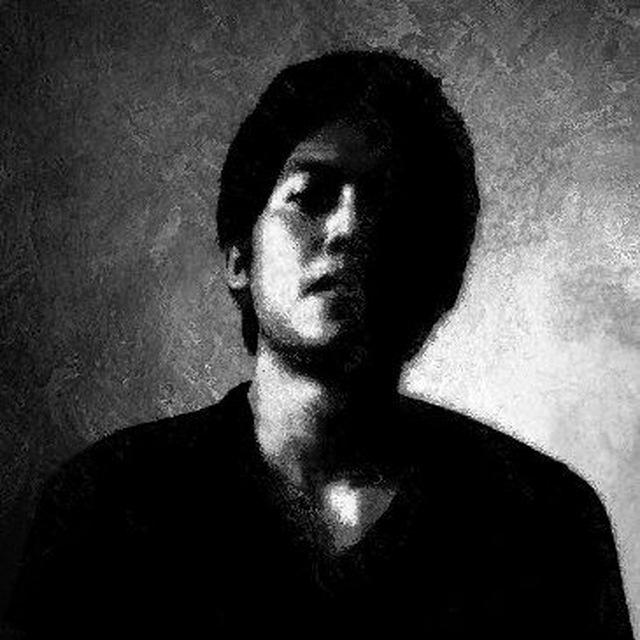
\includegraphics[width=6cm]{photo_diri.jpg}
  \captionof{figure}{Rizqi Nur Assyaufi, Jr Ruby Programmer}
  \label{gam:gambarsatu}
\end{minipage}\\

\textbf{Rizqi Nur Assyaufi}, seperti yang teman-teman lihat pada Gambar \ref{gam:gambarsatu}, memulai karirnya sebagai seorang Ruby programmer pada tahun 2019. Mengawali debutnya dengan bergabung pada \textit{software house} yang berbasis di Kuala Lumpur, Malaysia. Startup ini merupakan \textit{startup} yang berbasis \textit{remote}. Sehingga, pengalaman ini menjadi yang pertama kali baginya bekerja bersama programmer lain dari jarak jauh.

\end{document}
